\documentclass[logo,reportComp]{thesis}
\usepackage[cpp,pseudo,linenum,optidef]{mypackage}

\title{最优化理论期末报告}
\subtitle{}
\school{数据科学与计算机学院}
\author{陈鸿峥}
\classname{17大数据与人工智能}
\stunum{17341015}
\headercontext{最优化理论期末报告}
\lstset{language=python}

\begin{document}

\maketitle

\section{问题一}
\subsection{问题描述}
考虑线性测量$\vb=A\vx+\ve$,其中$\vb$为$50$维的测量值,$A$为$50\times 100$维的测量矩阵,$\vx$为$100$维的未知稀疏向量且稀疏度为$5$,$\ve$为$50$维的测量噪声。
从$\vb$与$A$中恢复$\vx$的一范数规范化,最小二乘模型如下:
\[\min\lrp{\frac{1}{2}\norm{A\vx-\vb}_2^2+p\norm{\vx}_1}\]
其中$p$为非负的正则化参数。

请设计下述算法求解该问题:
\begin{enumerate}
    \item 邻近点梯度下降法
    \item 交替方向乘子法
    \item 次梯度法
\end{enumerate}

在实验中,设$\vx$的真值中的非零元素服从均值为$0$方差为$1$的高斯分布,$A$中的元素服从均值为$0$方差为$1$的高斯分布,$\ve$中的元素服从均值为$0$方差为$0.1$的高斯分布。
对于每种算法,请给出每步计算结果与真值的距离以及每步计算结果与最优解的距离。
此外,请讨论正则化参数$p$对计算结果的影响。

\subsection{算法设计}
设
\begin{equation}
f(\vx)=\frac{1}{2}\norm{A\vx-\vb}_2^2+p\norm{\vx}_1
\end{equation}

\subsubsection{邻近点梯度下降法}
设
\[\begin{cases}
s(\vx):=\dfrac{1}{2}\norm{A\vx-\vb}_2^2\\
r(\vx):=p\norm{\vx}_1
\end{cases}\]
其中,$A\in\rr^{m\times n}$,$\vx\in\rr^n$,$\vb,\ve\in\rr^m$(在本题中$m=50,n=100$),$s(\vx)$为光滑函数,$r(\vx)$为非光滑函数,则原式
\[f(\vx)=s(\vx)+r(\vx)\]
先求$r(\vx)$的邻近点投影
\begin{equation}
\label{equ:prox}
\opprox \hat{\vx}=\argmin_\vx\lrp{p\norm{\vx}_1+\frac{1}{2\alpha}\norm{\vx-\hat{\vx}}_2^2}
\end{equation}
对(\ref{equ:prox})式右侧展开有
\begin{equation}
\label{equ:prox2}
\argmin_\vx\lrp{p\sum_{i=1}^n|x_i|+\frac{1}{2\alpha}\sum_{i=1}^n(x_i-\hat{x}_i)^2}
\end{equation}
注意到(\ref{equ:prox2})式对于下标$i$相互独立,故要求\ref{equ:prox2}的最小值,等价于对每一个下标$i$求最小值后求和,即
\begin{equation}
\label{equ:prox3}
\argmin_{x_i}\lrp{p|x_i|+\frac{1}{2\alpha}(x_i-\hat{x}_i)^2},\;\forall i
\end{equation}
由不可微函数的极值判断条件有
\begin{equation}
0\in\lrp{\partial_{x_i}p|x_i|+\frac{1}{\alpha}(x_i-\hat{x}_i)},\;\forall i
\end{equation}
对每一个$x_i$进行分类讨论
\begin{itemize}
	\item 若$x_i>0$,则$|x_i|$对于$|x_i|$可微,即$\partial_{x_i}|x_i|=1$,有
	\[p+\frac{1}{\alpha}(x_i-\hat{x}_i)=0\]
	整理得
	\[x_i=\hat{x}_i-\alpha p\]
	由于$x_i>0$,故$\hat{x}_i-\alpha p>0$,即$\hat{x}_i>\alpha p$
	\item 若$x_i<0$,则$|x_i|$对于$|x_i|$可微,即$\partial_{x_i}|x_i|=-1$,有
	\[-p+\frac{1}{\alpha}(x_i-\hat{x}_i)=0\]
	整理得
	\[x_i=\hat{x}_i+\alpha p\]
	由于$x_i<0$,故$\hat{x}_i+\alpha p<0$,即$\hat{x}_i<-\alpha p$
	\item 若$x_i=0$,则$|x_i|$对于$|x_i|$不可微,需要求次梯度,$\partial_{x_i}|x_i|=[-1,1]$,即
	\[0\in\left[-p-\frac{\hat{x}_i}{\alpha},p-\frac{\hat{x}_i}{\alpha}\right]\]
	那么,需要满足
	\[\begin{cases}
	p-\dfrac{\hat{x}_i}{\alpha}\geq 0\\
	-p-\dfrac{\hat{x}_i}{\alpha}\leq 0
	\end{cases}\]
	推得
	\[\hat{x}_i\in[-\alpha p,\alpha p]\]
\end{itemize}
综上,有
\begin{equation}
\label{equ:soft-thresholding}
x_i=\begin{cases}
\hat{x}_i+\alpha p & \hat{x}_i<-\alpha p\\
0 & \hat{x}_i\in[-\alpha p,\alpha p]\\
\hat{x}_i-\alpha p & \hat{x}_i>\alpha p
\end{cases}
\end{equation}
可以得到图\ref{fig:soft-thresholding}的软门限(soft-thresholding)曲线
\begin{figure}[H]
\centering
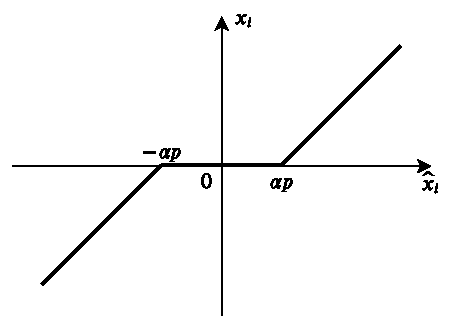
\includegraphics[width=0.5\linewidth]{fig/soft-thresholding.pdf}
\caption{关于$x_i$与$\hat{x}_i$的软门限图}
\label{fig:soft-thresholding}
\end{figure}

进一步,得到邻近点梯度下降法的迭代式如下
\begin{equation}
\begin{cases}
\iter{\vx}{k+\frac{1}{2}}=\iter{\vx}{k}-\alpha\nabla s(\iter{\vx}{k})=\iter{\vx}{k}-\alpha A^T(A\iter{\vx}{k}-\vb)\\
\iter{\vx}{k+1}=\opprox \iter{\vx}{k+\frac{1}{2}}=\argmin_\vx\lrp{p\norm{\vx}_1+\dfrac{1}{2\alpha}\norm{\vx-\iter{\vx}{k+\frac{1}{2}}}_2^2}
\end{cases}
\end{equation}
其中,$\iter{x}{k+\frac{1}{2}}$可直接计算,$\iter{x}{k+1}$的显式解可由(\ref{equ:soft-thresholding})式求得。

\subsubsection{交替方向乘子法}
对原问题进行变形,等价于下述约束问题
\begin{mini*}
{}{\frac{1}{2}\norm{A\vx-\vb}_2^2+p\norm{\vy}_1}{}{}
\addConstraint{\vx-\vy}{=0}
\end{mini*}

构造增广拉格朗日函数
\begin{equation}
\label{equ:clagrange}
L_c(\vx,\vy,\vv)=\frac{1}{2}\norm{A\vx-\vb}_2^2+p\norm{\vy}_1+\vv^\T(\vx-\vy)+\frac{c}{2}\norm{\vx-\vy}_2^2
\end{equation}

可以得到交替方向乘子法的迭代格式
\begin{equation}
\label{equ:admm1}
\begin{cases}
\iter{\vx}{k+1}=\argmin_\vx L_c(\vx,\iter{\vy}{k},\iter{\vv}{k})\\
\iter{\vy}{k+1}=\argmin_\vy L_c(\iter{\vx}{k+1},\vy,\iter{\vv}{k})\\
\iter{\vv}{k+1}=\iter{\vv}{k}+c(\iter{\vx}{k+1}-\iter{\vy}{k+1})
\end{cases}
\end{equation}

对$\iter{\vx}{k+1}$展开并配方,并将非主元项忽略,可求得(\ref{equ:admm1})式与下面的式子等价
\begin{subequations}
\begin{numcases}{}
\iter{\vx}{k+1}=\argmin_\vx \lrp{\frac{1}{2}\norm{A\vx-\vb}_2^2+\frac{c}{2}\norm{\vx-\iter{\vy}{k}+\frac{\iter{\vv}{k}}{c}}_2^2}\label{equ:admm21}\\
\iter{\vy}{k+1}=\argmin_\vy \lrp{p\norm{\vy}_1+\frac{c}{2}\norm{\iter{\vx}{k+1}-\vy+\frac{\iter{\vv}{k}}{c}}_2^2}\label{equ:admm22}\\
\iter{\vv}{k+1}=\iter{\vv}{k}+c(\iter{\vx}{k+1}-\iter{\vy}{k+1})\label{equ:admm23}
\end{numcases}
\end{subequations}

对于(\ref{equ:admm21})式,可直接通过求梯度的方法得到显式解,得到
\[\iter{\vx}{k+1}=(A^\T A+cI)^{-1}(A^\T\vb+c\iter{\vy}{k}-\iter{\vv}{k})\]
对于(\ref{equ:admm22})式,由于涉及一范数,故需要求次微分,类似(\ref{equ:soft-thresholding})式的方法,设$z_i=\iter{x}{k+1}_i+\dfrac{\iter{v}{k}_i}{c}$,可得到类似的软门限表达式
\[y_i=\begin{cases}
z_i-\dfrac{p}{c} & z_i>\dfrac{p}{c}\\
0 & z_i\in\lrs{-\dfrac{p}{c},\dfrac{p}{c}}\\
z_i+\dfrac{p}{c} & z_i<-\dfrac{p}{c}
\end{cases}\]

进而可以通过(\ref{equ:admm21})(\ref{equ:admm22})(\ref{equ:admm23})式迭代求解。

\subsubsection{次梯度法}
对原式直接求次梯度有
\begin{equation}
\partial f(\vx)=A^\T(A\vx-\vb)+p\partial\norm{\vx}_1
\end{equation}
其中
\[(\partial\norm{\vx}_1)_i=\partial|x_i|=
\begin{cases}
1 & x_i>0\\
[-1,1] & x_i=0\\
-1 & x_i<0
\end{cases}\]

进而可以直接得到次梯度法的迭代格式
\begin{equation}
\iter{\vx}{k+1}=\iter{\vx}{k}-\alpha\partial f(\iter{\vx}{k})
\end{equation}

\subsection{数值实验}
采用Python进行编程\footnote{使用numpy进行数值计算,matplotlib进行画图},对上述三种方法进行迭代计算,直到精度达到$10^{-8}$。

完整代码请见\verb'p1.py'文件,这里只截取核心代码部分。

邻近点梯度法如下,设超参数$\alpha=10^{-3}$。
\begin{lstlisting}
class ProximalGradient():

	def __init__(self, alpha=1e-3):
		self.name = "Proximal Gradient"
		self.alpha = alpha

	def soft_thresholding(self, x, offset):
		if x < (-1) * offset:
			return x + offset
		elif x > offset:
			return x - offset
		else:
			return 0

	def prox(self, xk_old, offset):
		# v_soft_thresholding = np.vectorize(self.soft_thresholding)
		# return v_soft_thresholding(xk_old,offset)
		xk_new = np.zeros(xk_old.size)
		for i in range(xk_old.size):
			xk_new[i] = self.soft_thresholding(xk_old[i],offset)
		return xk_new

	def train(self,A,b,p):
		_, self.n = A.shape
		self.xk = np.zeros(self.n)

		res = []
		t = 0
		while True:
			xhat = self.xk - self.alpha * np.dot(A.T, np.dot(A, self.xk) - b)
			xk_new = self.prox(xhat, self.alpha * p)
			if np.linalg.norm(xk_new - self.xk, ord=2) < accuracy:
				break
			res.append(xk_new)
			self.xk = xk_new.copy()
			t += 1

		print(t)
		return self.xk, res
\end{lstlisting}

交替方向乘子法如下,设超参数$c=10^{-3}$。
\begin{lstlisting}
class ADMM():

	def __init__(self, c=1e-3):
		self.name = "ADMM"
		self.c = c

	def soft_thresholding(self, x, offset):
		if x < (-1) * offset:
			return x + offset
		elif x > offset:
			return x - offset
		else:
			return 0

	def prox(self, xk_old, offset):
		xk_new = np.zeros(xk_old.size)
		for i in range(xk_old.size):
			xk_new[i] = self.soft_thresholding(xk_old[i],offset)
		return xk_new

	def train(self,A,b,p):
		_, self.n = A.shape
		self.xk = np.zeros(self.n)
		self.yk = np.zeros(self.n)
		self.vk = np.zeros(self.n)

		res = []
		t = 0
		while True:
			xk_new = np.dot(
				np.linalg.inv(np.dot(A.T, A) + self.c * np.eye(self.n,self.n)),
				np.dot(A.T, b) + self.c * self.yk - self.vk)
			self.yk = self.prox(xk_new + self.vk / self.c, p / self.c)
			self.vk = self.vk + self.c * (xk_new - self.yk)
			if np.linalg.norm(xk_new - self.xk, ord=2) < accuracy:
				break
			res.append(xk_new)
			self.xk = xk_new.copy()
			t += 1

		print(t)
		return self.xk, res
\end{lstlisting}

次梯度法如下,采用递减步长$\iter{\alpha}{k+1}=\iter{\alpha}{0}/(k+1)$,初始步长$\iter{\alpha}{0}=10^{-3}$。
\begin{lstlisting}
class Subgradient():

	def __init__(self,alpha=1e-3):
		self.name = "Subgradient"
		self.alpha = alpha

	def subgrad(self,x):
		# subgradient of |x|
		pdx = np.zeros(x.size)
		for i in range(x.size):
			if x[i] != 0:
				pdx[i] = 1 if x[i] > 0 else -1
			else: # pick a random float from [-1,1]
				pdx[i] = 2 * np.random.random() - 1
		return pdx

	def train(self,A,b,p):
		_, self.n = A.shape
		self.xk = np.zeros(self.n)

		res = []
		t = 0
		while True:
			alphak = self.alpha / (t + 1) # remember to decay the step
			pdf = np.dot(A.T, np.dot(A, self.xk) - b) + self.subgrad(self.xk)
			xk_new = self.xk - alphak * pdf
			if np.linalg.norm(xk_new - self.xk, ord=2) < accuracy:
				break
			res.append(xk_new)
			self.xk = xk_new.copy()
			t += 1

		print(t)
		return self.xk, res
\end{lstlisting}

\subsection{结果分析}
% 横轴迭代次数$k$,纵轴对数坐标,\norm{\iter{x}{k}-\iter{x}{t}}_2^2, \norm{\iter{x}{k}-x^\star}_2^2
记最优解$\vx^\star$为最后一次迭代获得的$\vx$值,真值为$\vx_{\text{true}}$。

运行结果如图\ref{fig:proxgrad}、图\ref{fig:admm}和图\ref{fig:subgrad}所示,该次实验$p=0.1$。

\begin{minipage}{0.5\linewidth}
\begin{figure}[H]
\centering
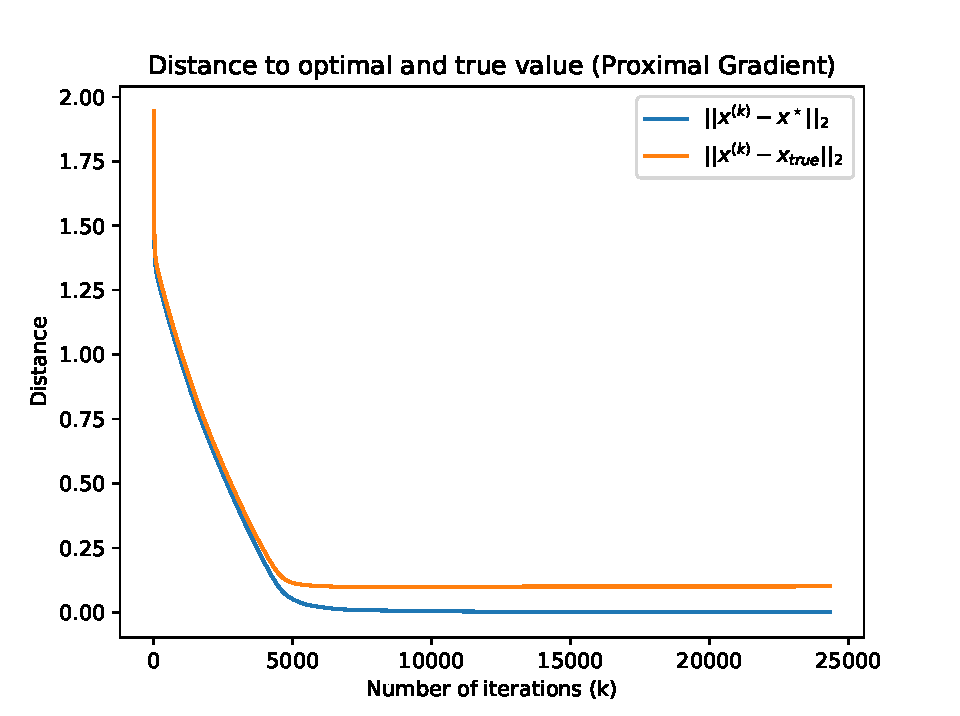
\includegraphics[width=\linewidth]{fig/proxgrad.pdf}
\caption{邻近点梯度下降法}
\label{fig:proxgrad}
\end{figure}
\end{minipage}
\begin{minipage}{0.5\linewidth}
\begin{figure}[H]
\centering
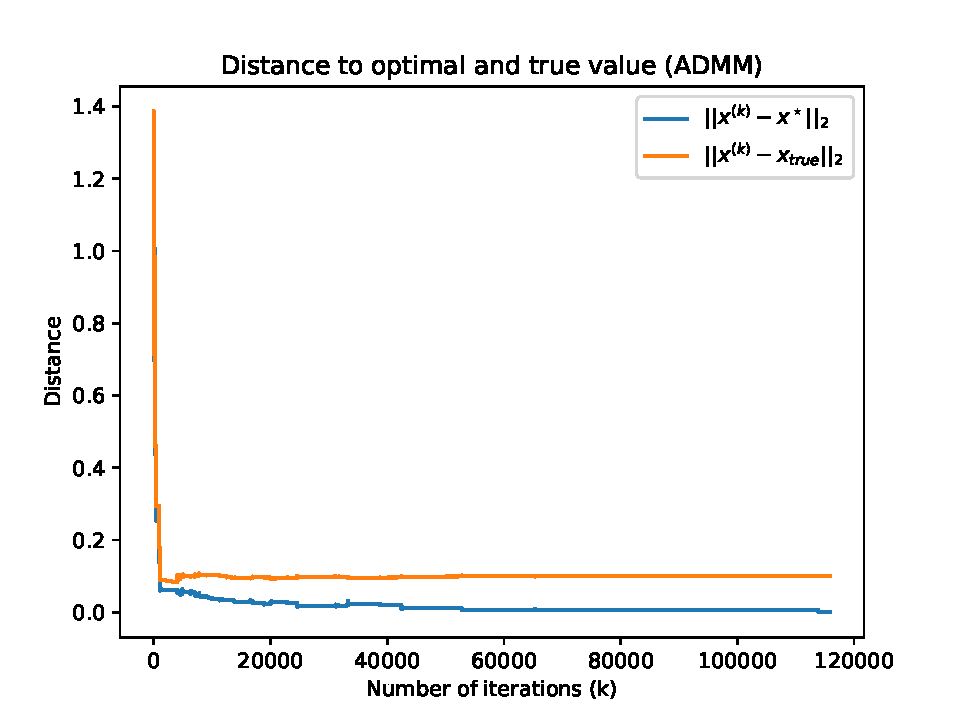
\includegraphics[width=\linewidth]{fig/admm.pdf}
\caption{交替方向乘子法}
\label{fig:admm}
\end{figure}
\end{minipage}
\begin{figure}[H]
\centering
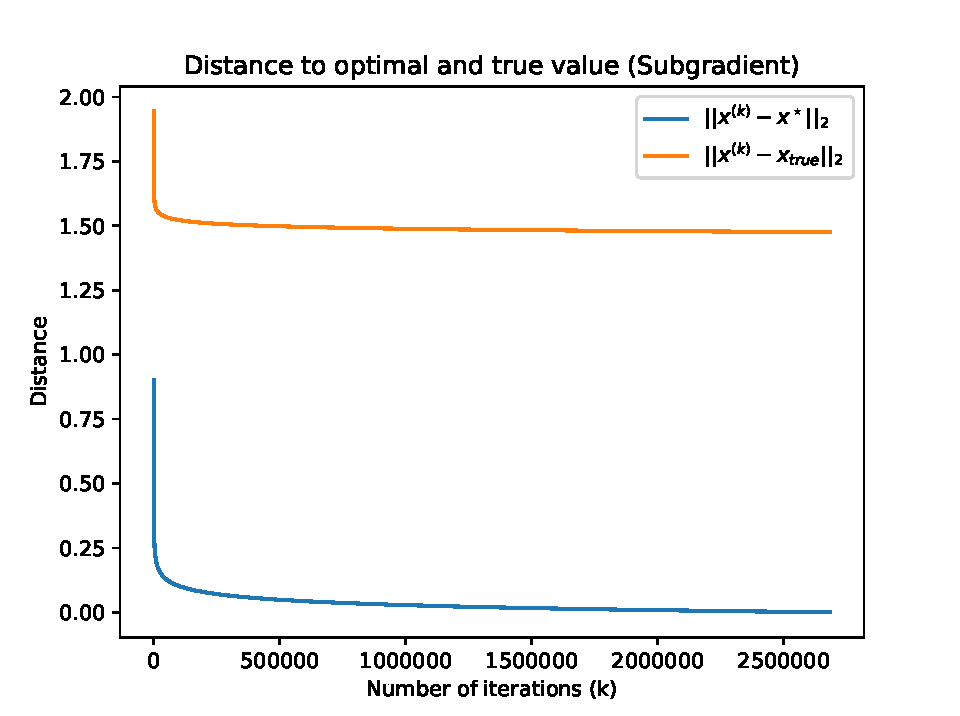
\includegraphics[width=0.5\linewidth]{fig/subgrad.pdf}
\caption{次梯度法}
\label{fig:subgrad}
\end{figure}

由实际的运行时间可以得出,邻近点梯度法和交替方向乘子法达到目标精度需要的时间都比较短,次梯度法所需的时间最长。
从迭代的次数也可以看出,邻近点梯度下降法需要$24349$轮迭代,交替方向乘子法需要$115901$轮迭代,次梯度法需要$2684797$轮迭代,都相差了一个数量级。
(此实验仅仅展示了一种情况,实际上迭代次数与超参数的选择有关,见下面的实验。)

不仅如此,从上述三幅图中还可以看出,交替方向乘子法和邻近点梯度下降法都能达到很高的精度(即与真值相差不多),且收敛速度快,但次梯度法迭代次数多且精度非常低,是一种非常糟糕的算法。

关于正则化参数$p$对最终结果的影响可见图\ref{fig:pprox}、图\ref{fig:padmm}和图\ref{fig:psubgrad}。
\begin{figure}[H]
\centering
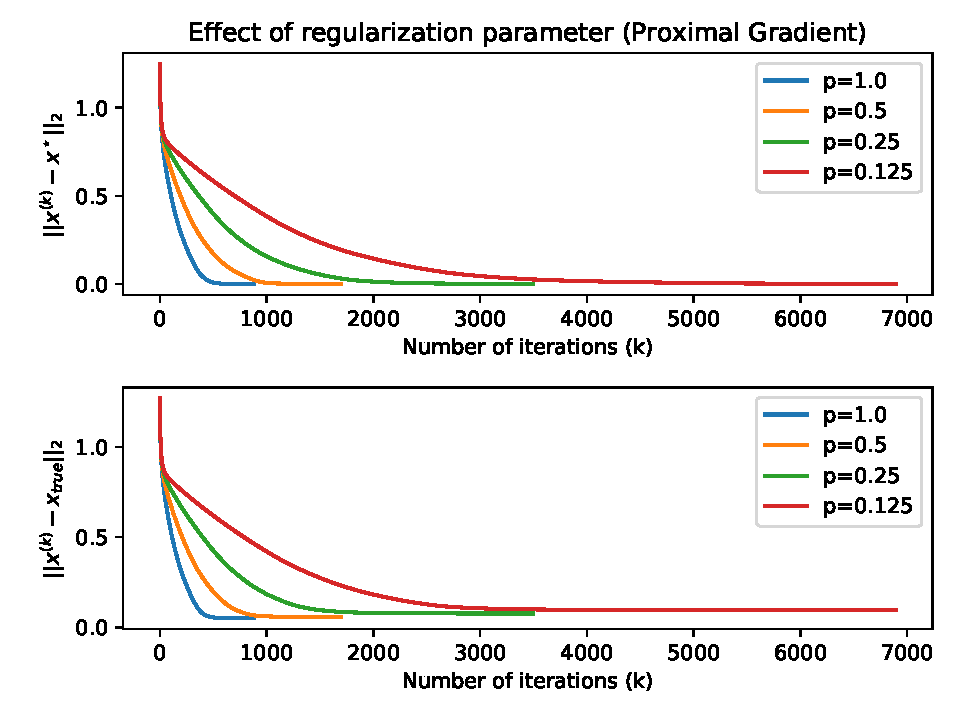
\includegraphics[width=0.8\linewidth]{fig/pprox.pdf}
\caption{邻近点梯度下降法}
\label{fig:pprox}
\end{figure}
\begin{figure}[H]
\centering
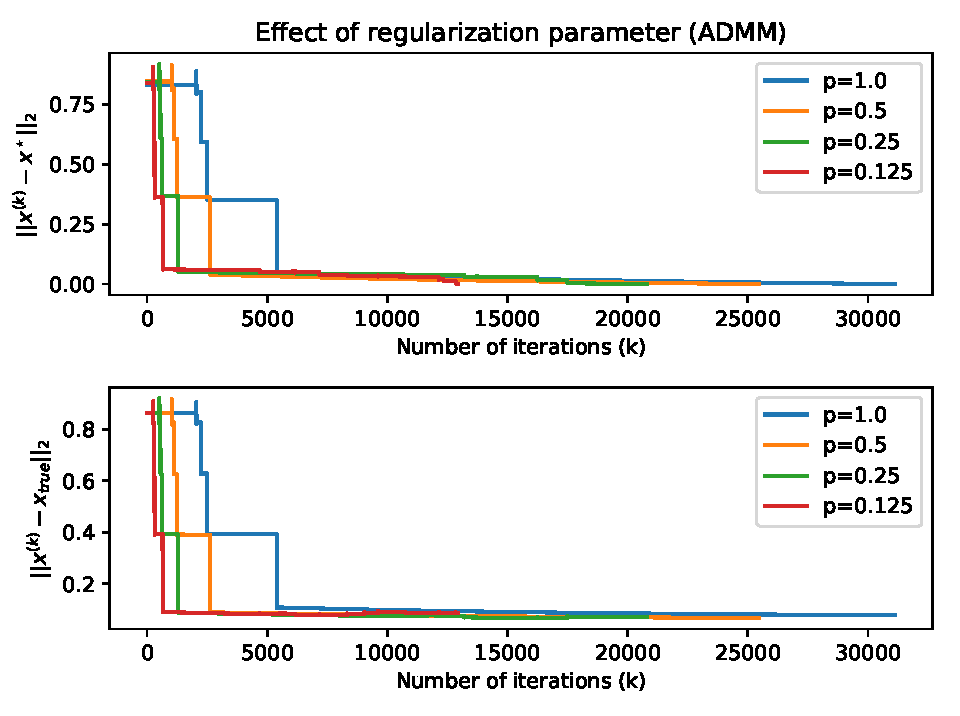
\includegraphics[width=0.8\linewidth]{fig/padmm.pdf}
\caption{交替方向乘子法}
\label{fig:padmm}
\end{figure}
\begin{figure}[H]
\centering
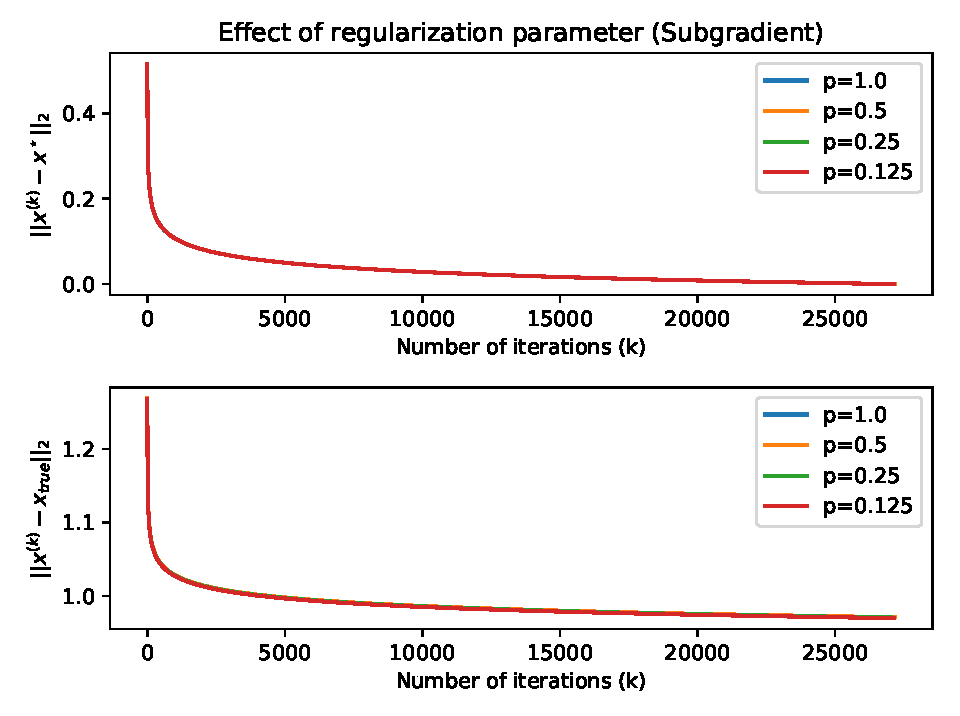
\includegraphics[width=0.8\linewidth]{fig/psubgrad.pdf}
\caption{次梯度法}
\label{fig:psubgrad}
\end{figure}

从这三幅图中可以看出,当正则化参数$p$对迭代次数和收敛精度都有一定的影响。
对于邻近点梯度法,$p$取较大的值时,收敛速度比较快,且精度也较高。
对于交替方向乘子法,$p$取较小的值时,收敛速度较快,但精度差异没有邻近点梯度法那么明显。
而对于次梯度法,$p$对收敛速度和收敛精度几乎没有影响。


\section{问题二}
\subsection{问题描述}
请设计下述算法,求解MNIST数据集上的Logistic Regression问题:
\begin{enumerate}
    \item 梯度下降法
    \item 随机梯度法
\end{enumerate}

对于每种算法,请给出每步计算结果与最优解的距离以及每步计算结果在测试集上所对应的分类精度。
此外,请讨论随机梯度法中Mini Batch大小对计算结果的影响。

可参考:\url{http://deeplearning.net/tutorial/logreg.html}

\subsection{算法设计}
由于MNIST手写数据集为多分类问题,需要将输入的图片映射到对应的$10$个数字上,故采用多类别的logistic回归,即softmax回归进行求解。
% multiclass logistic regression. Other common names for it include softmax regression and multinomial regression

设训练集$\{(\vx_i,y_i)\}_{i=1}^M$,其中$M$为训练集数目,${|\mathcal{C}|}$为类别数目,$\vx_i\in\rr^{n+1}$为输入样本,$y_i\in\{0,1,\ldots,|\mathcal{C}|-1\}$为对应的标签。
在本问题中${|\mathcal{C}|}=10$,$M=60000$,$n=28\times 28=784$,这里已经将二维的图片数组展平为一维的向量。

输入$\vx_i$属于第$y_i$类的条件概率可用softmax函数进行计算
\begin{equation}
p(y_i\mid \vx_i;W)=\frac{\ee^{\vw_{y_i}^\T\vx_i}}{\sum_{c=0}^{|\mathcal{C}|-1}\ee^{\vw_c^\T\vx_i}}
\end{equation}
其中,
\[W=\bmat{\vw_0^\T\\\vw_1^\T\\\vdots\\\vw_{|\mathcal{C}|-1}^\T}\in\rr^{{|\mathcal{C}|}\times (n+1)}\]
为需要训练的参数,$\vw_i\in\rr^{n+1}$为每一个类别对应的权重向量\footnote{注意到$\vw^\T\vx+b=\bmat{\vw^\T & b}\bmat{\vx\\1}$,故将最后的偏置项归入$\vw$中,并在$\vx$中添加为$1$的一个维度,进而偏置量和权重可以一起运算,$\vw_c^\T$和$\vx_i$都有$n+1$个维度。}。

从而得到数据集的似然函数为
\[\mL(Y\mid X;W)=\prod_{i=1}^m p(y_i\mid\vx_i;W)\]
对应的对数似然函数为
\[\ln\mL(Y\mid X;W)=\sum_{i=1}^m\ln p(y_i\mid\vx_i;W)\]

极大化对数似然函数,相当于极小化负对数似然函数(negative log likelihood, NLL)\footnote{由于已经取了softmax函数,并且在实施时采用独热码(one-hot encoding)方便矩阵运算,所以这里的NLL也可以看作是交叉熵函数。},故得到最优化问题
\begin{equation}
\min_W \;\ell(W):=-\ln\mL(Y\mid X;W)
\end{equation}
$\ell(W)$其实也是深度学习领域常说的损失函数(loss)。

对$\ln p(y_i\mid\vx_i;W)$求梯度,有
\[\pd{\ln p(y_i\mid\vx_i;W)}{\vw_j}=
\begin{cases}
\vx(1-p(y_i\mid\vx_i;W)) & y_i=j\\
\vx p(y_i\mid\vx_i;W) & y_i\ne j
\end{cases},\;j\in\{0,1,\ldots,|\mathcal{C}|-1\}\]
进而
\begin{equation}
\nabla_{\vw_j}\ell(W)=-\sum_{i=1}^m\lrs{\vx_i\lrp{\vone(y_i=j)-p(y_i\mid\vx_i;W)}}
\end{equation}
其中,$\vone(\cdot)$为示性函数,当输入为真时返回$1$,输入为假时返回$0$。

最终得到梯度下降的表达式
\begin{equation}
\label{equ:gd}
\iter{\vw}{k+1}_j=\iter{\vw}{k}_j-\frac{\iter{\alpha}{k}}{m}\nabla_{\vw_j}\ell(W)
\end{equation}
其中,$m$为小批量大小。
当$m$选取不同值时,(\ref{equ:gd})式为不同的优化方法:
\begin{itemize}
\item 当$m=M$时,梯度下降法,每次选取\textbf{所有样本}用于更新权重
\item 当$m=1$时,随机梯度下降法(SGD),每次选取\textbf{一个样本}用于更新权重
\item 当$m\in[2,M-1]$时,小批量梯度下降法,每次只选取\textbf{部分样本}用于更新权重
\end{itemize}

\subsection{数值实验}
注意本作业的所有实验都\textbf{没有}调用额外的深度学习框架,仅仅使用了Python内置的库及numpy进行数值计算。
MNIST输入数据以numpy压缩格式存储,从\url{https://s3.amazonaws.com/img-datasets/mnist.npz}获取。
可从中直接读出\verb'x_train'、\verb'y_train'、\verb'x_test'和\verb'y_test'。

值得一提的几个实现细节:
\begin{itemize}
	\item 读入\verb'x_train'和\verb'x_test'后,增加一个全为$1$的维度,用于与偏移量$b$点乘
	\item 训练前先进行归一化(normalization)防止计算softmax时数值上溢(overflow) % https://shusei-e.github.io/deep%20learning/softmax_without_overflow/
	\item 充分利用了numpy的广播(broadcast)、扩展(keepdim)等技巧,使得梯度计算可以直接运用矩阵乘法,而不需逐元素相乘
	\item 步长/学习率设置为$\alpha=0.1$
\end{itemize}

核心代码如下,完整代码请见\verb'p2.py'。
\begin{lstlisting}
class SoftmaxRegression():

	def train(self, X, y_true, n_classes, n_iters=10, learning_rate=0.1, batch_size=1):
		self.n_samples, n_features = X.shape # (M, C)
		self.n_classes = n_classes
		self.batch_size = batch_size
		self.weights = np.random.rand(self.n_classes, n_features)
		all_losses = []
		all_accuracy = []
		all_weights = []
		
		for i in range(n_iters):
			batch_index = np.array(random.sample(range(self.n_samples),self.batch_size))
			X_batch, y_batch = X[batch_index], y_true[batch_index]
			scores = self.compute_scores(X_batch) # w^T.x
			probs = self.softmax(scores)
			y_one_hot = self.one_hot(y_batch)

			loss = self.nll_loss(y_one_hot, probs) # target function
			all_losses.append(loss)

			# gradient descent -> update weights
			old_weights = self.weights.copy()
			dw = (1 / self.batch_size) * np.dot(X_batch.T, (probs - y_one_hot))
			self.weights = self.weights - learning_rate * dw.T
			all_weights.append(self.weights)

			if i % 100 == 0 or i == n_iters - 1:
				y_predict = self.predict(X_test)
				all_accuracy.append((np.sum(y_predict == y_test) / X_test.shape[0]) * 100)
				print(f'Iteration number: {i}, loss: {np.round(loss, 4)}, accuracy: {all_accuracy[-1]}%')

		return all_weights, all_losses, all_accuracy

	def predict(self, X):
		scores = self.compute_scores(X)
		probs = self.softmax(scores)
		return np.argmax(probs, axis=1)[:, np.newaxis]

	def softmax(self, scores):
		exp = np.exp(scores) # (n_samples, n_classes)
		sum_exp = np.sum(np.exp(scores), axis=1, keepdims=True) # sum along classes
		softmax = exp / sum_exp
		return softmax

	def compute_scores(self, X):
		# X: (n_samples, n_features)
		# scores: (n_samples, n_classes)
		return np.dot(X, self.weights.T)

	def nll_loss(self, y_true, probs):
		loss = - (1 / self.batch_size) * np.sum(y_true * np.log(probs))
		return loss

	def one_hot(self, y):
		one_hot = np.zeros((y.size, self.n_classes))
		one_hot[np.arange(y.size), y.T] = 1
		return one_hot
\end{lstlisting}

\subsection{结果分析}
\begin{minipage}{0.5\linewidth}
\begin{figure}[H]
\centering
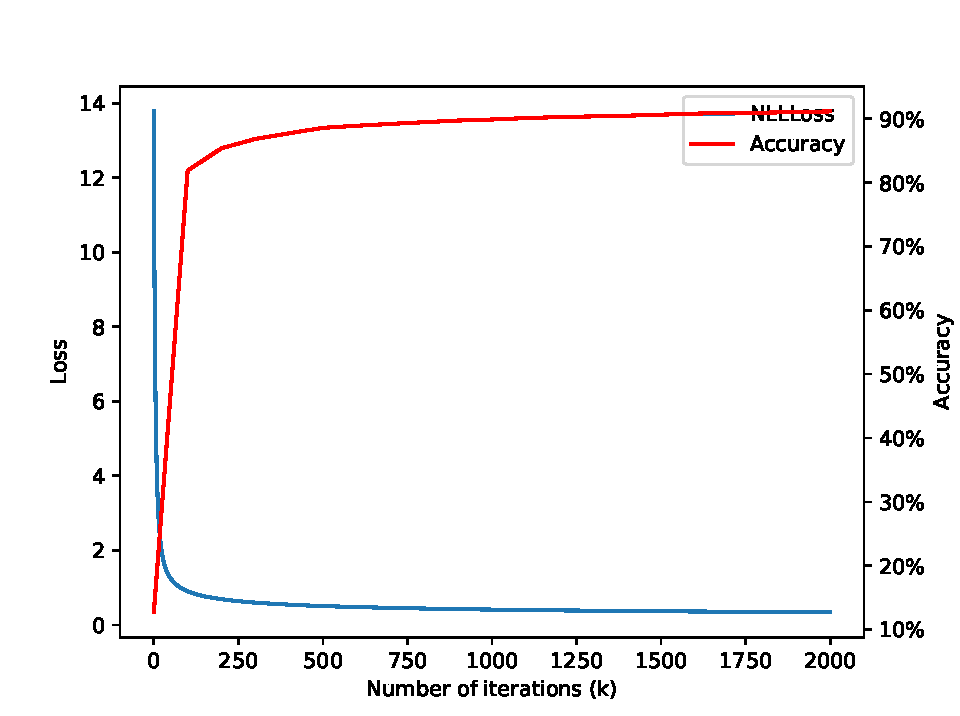
\includegraphics[width=\linewidth]{fig/p2-acc.pdf}
\caption{梯度下降法损失函数及分类精度变化}
\label{fig:p2-acc-gd}
\end{figure}
\end{minipage}
\begin{minipage}{0.5\linewidth}
\begin{figure}[H]
\centering
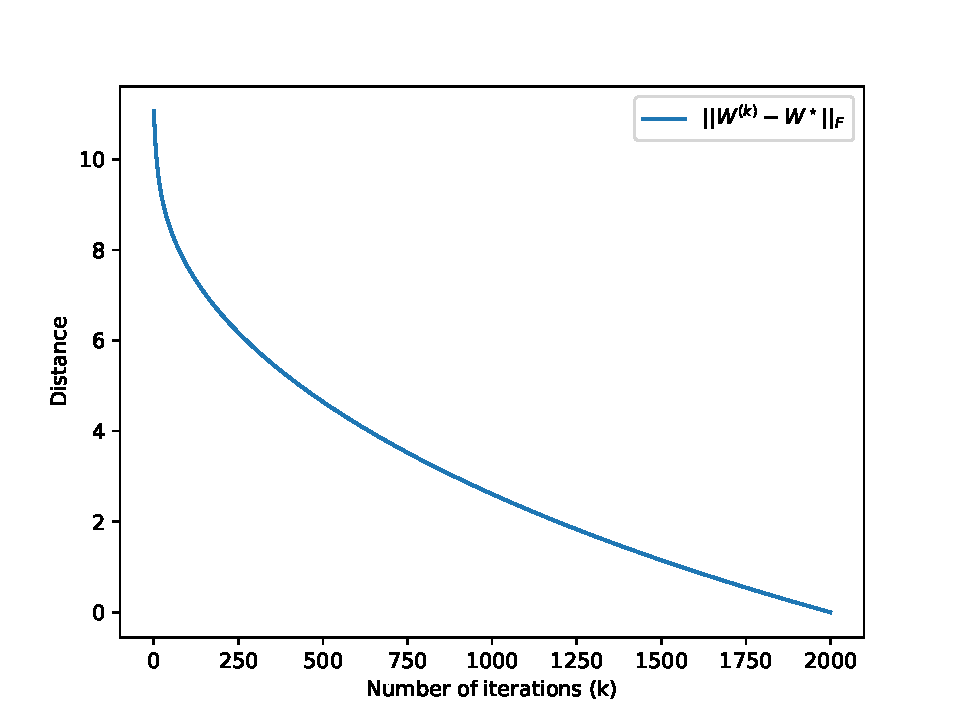
\includegraphics[width=\linewidth]{fig/p2-opt-dist.pdf}
\caption{梯度下降法与最优解的距离变化}
\label{fig:p2-opt-dist-gd}
\end{figure}
\end{minipage}
\begin{minipage}{0.5\linewidth}
\begin{figure}[H]
\centering
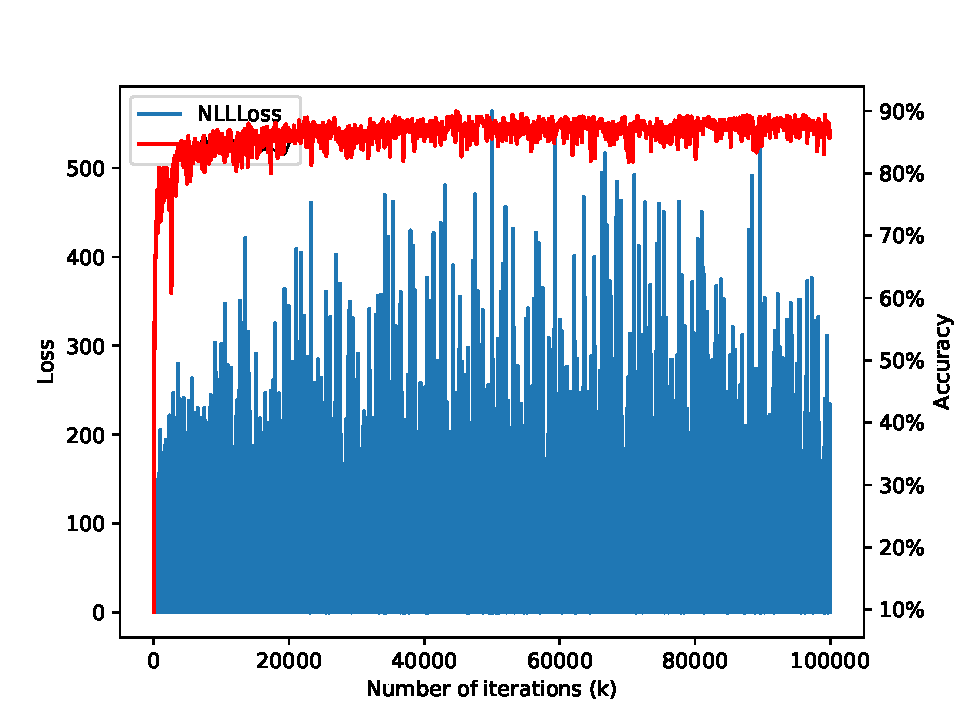
\includegraphics[width=\linewidth]{fig/p2-sgd-acc.pdf}
\caption{SGD损失函数及分类精度变化}
\label{fig:p2-acc-sgd}
\end{figure}
\end{minipage}
\begin{minipage}{0.5\linewidth}
\begin{figure}[H]
\centering
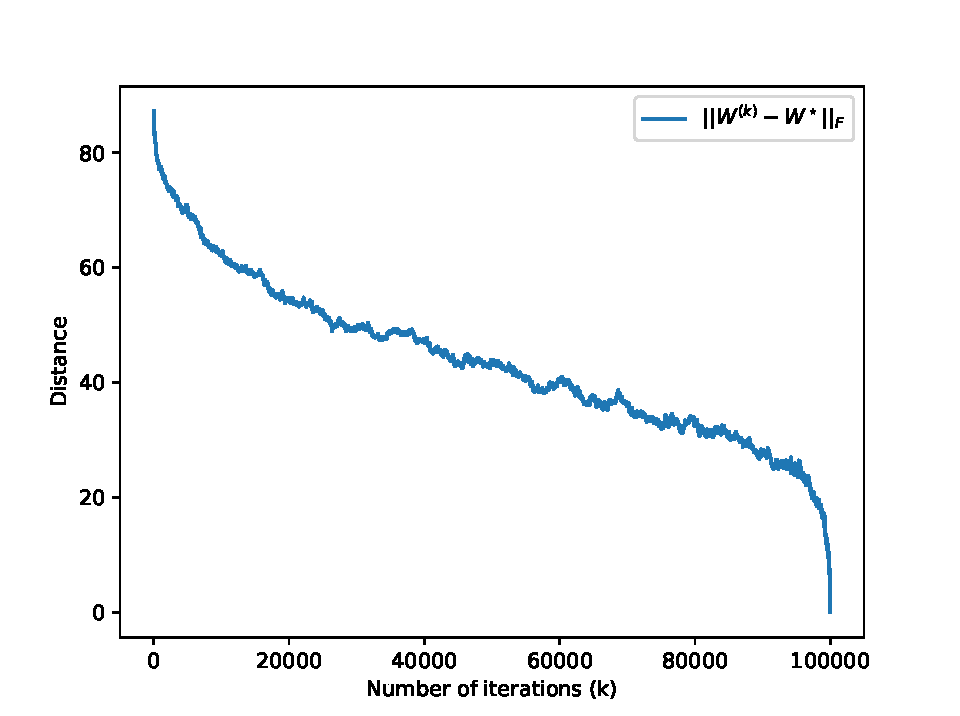
\includegraphics[width=\linewidth]{fig/p2-sgd-opt-dist.pdf}
\caption{SGD与最优解的距离变化}
\label{fig:p2-opt-dist-sgd}
\end{figure}
\end{minipage}

从图\ref{fig:p2-acc-gd}中可以看出,运用梯度下降法求解,损失函数不断下降,在测试集上的分类精度不断上升;图\ref{fig:p2-opt-dist-gd}中可以看出,迭代过程确实是在往最优解方向逼近\footnote{注:这里采用了矩阵的F范数作为距离度量。},最终收敛在91.4\%的精度(迭代2000次)。

同样,从图\ref{fig:p2-acc-sgd}和图\ref{fig:p2-opt-dist-sgd}中也可以得出对随机梯度下降法同样的结论,但是随机梯度下降法明显要不稳定得多,分类精度与损失函数都有较大波动(因为受单一特殊样本影响非常大),最终达到88\%左右的精度(迭代60000次),没有梯度下降法优。

批量大小、精度和训练时间的比较如表\ref{tab:minibatch}所示。
从表中可以看出,当\verb'batch_size'较小时,参数更新的速度快,但不稳定/较难收敛,最终达到的精度往往较低。
而\verb'batch_size'较大时,迭代速度非常慢,但往往几轮迭代就能得到很好的效果,而且随着迭代轮数的不断增加,分类的精度也不断在提升。
注意由于限制了最大迭代次数,所以对于比较大的\verb'batch_size'其损失函数依然在下降,即未收敛到最优解。
尽管其能达到更高的精度(91.31\%以上),但是其所花费的时间显然是不能让人接受的。
如此例中,100到1000之间的\verb'batch_size'就是比较好的选择。
\begin{table}[H]
\caption{批量大小、精度和训练时间的比较}
\label{tab:minibatch}
\centering
\begin{tabular}{|c|c|c|c|}\hline
\textbf{批量大小} & \textbf{迭代次数} & \textbf{分类精度} & \textbf{训练时间}\\\hline
1 & 10000 & 86.67\% & 2.38s\\\hline
10 & 10000 & 88.08\% & 3.21s\\\hline
100 & 5000 & 91.04\% & 2.97s\\\hline
1000 & 5000 & 91.63\% & 38.81s\\\hline
10000 & 1000 & 89.46\% & 69.88s\\\hline
60000 & 1000 & 89.86\% & 404.68s\\\hline
1 & 2500 & 82.6\% & 0.58s\\\hline
10 & 2500 & 87.69\% & 0.64s\\\hline
100 & 2500 & 91.0\% & 1.30s\\\hline
1000 & 2500 & 91.31\% & 17.64s\\\hline
10000 & 2500 & 90.89\% & 170.88s\\\hline
60000 & 2500 & 90.88\% & 1010.26s\\\hline
\end{tabular}
\end{table}

图\ref{fig:batch-size}展示了批量大小(\verb'batch_size')对最终分类精度的影响。
我们也可以得到同样的结论,因此\verb'batch_size'的选取一定要适中,太小影响精度,太大影响训练时间。
通过多个参数的测试,就能快速找到比较合适的\verb'batch_size',进而加速训练并且训练的模型具有非常好的性能。
\begin{figure}[H]
\centering
\begin{tabular}{cc}
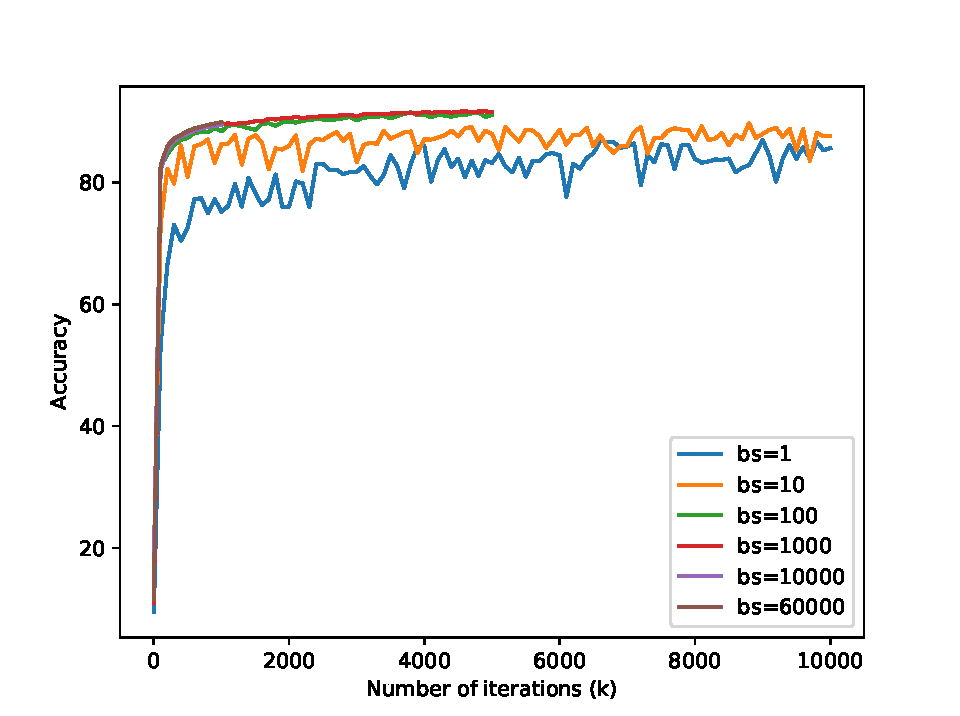
\includegraphics[width=0.5\linewidth]{fig/batch-size.pdf}
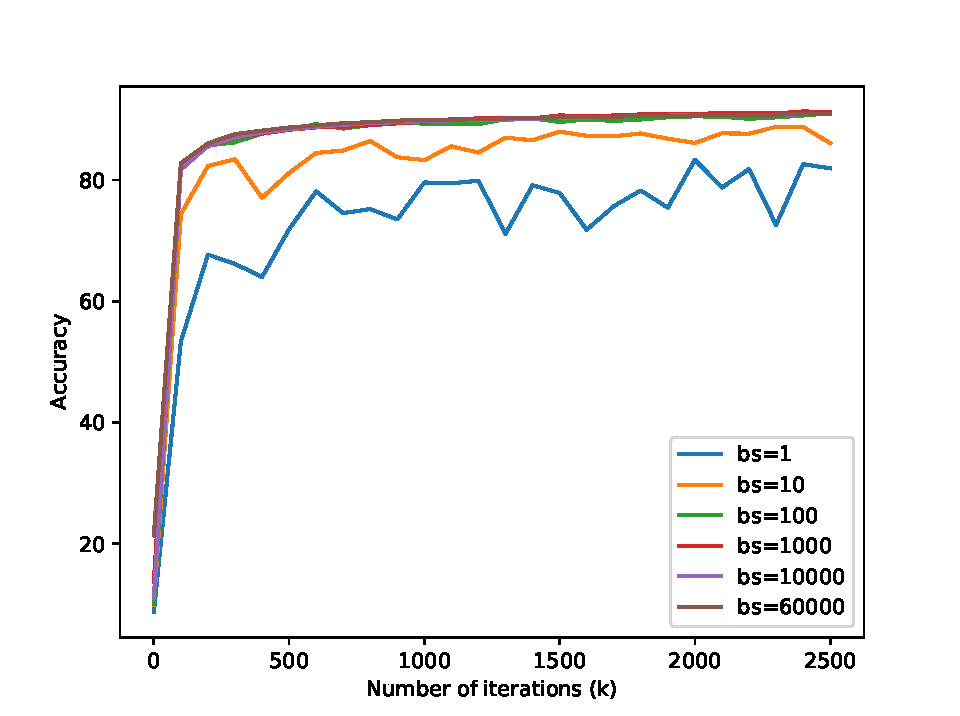
\includegraphics[width=0.5\linewidth]{fig/batch-size-2.pdf}
\end{tabular}
\caption{批量大小对分类精度的影响}
\label{fig:batch-size}
\end{figure}

\section{参考资料}
\begin{enumerate}
	\item Stanford CS231n, \url{http://cs231n.github.io/}
	\item Stanford UFLDL Tutorial - Softmax Regression, \url{http://deeplearning.stanford.edu/tutorial/supervised/SoftmaxRegression/}
\end{enumerate}
% http://yann.lecun.com/exdb/mnist/
% logistic回归,梯度下降法,牛顿法/IRLS算法 - RookieJ的文章 - 知乎 https://zhuanlan.zhihu.com/p/67842740
% https://github.com/zotroneneis/machine_learning_basics/blob/master/softmax_regression.ipynb
% https://blog.csdn.net/a19990412/article/details/85247465
% https://cntk.ai/pythondocs/CNTK_103B_MNIST_LogisticRegression.html

\end{document}

% 实验要求:
% 1、撰写并提交完整的实验报告,包括问题描述、算法设计、数值实验、结果分析。
% 2、编写并提交完整的源代码,建议用 MATLAB 实现。
% 3、2019 年 6 月 14 日(星期五)前提交至optimization_2019@163.com,要回信!